
%% ****** Start of file apstemplate.tex ****** %
%%
%%
%%   This file is part of the APS files in the REVTeX 4 distribution.
%%   Version 4.1r of REVTeX, August 2010
%%
%%
%%   Copyright (c) 2001, 2009, 2010 The American Physical Society.
%%
%%   See the REVTeX 4 README file for restrictions and more information.
%%
%
% This is a template for producing manuscripts for use with REVTEX 4.0
% Copy this file to another name and then work on that file.
% That way, you always have this original template file to use.
%
% Group addresses by affiliation; use superscriptaddress for long
% author lists, or if there are many overlapping affiliations.
% For Phys. Rev. appearance, change preprint to twocolumn.
% Choose pra, prb, prc, prd, pre, prl, prstab, prstper, or rmp for journal
%  Add 'draft' option to mark overfull boxes with black boxes
%  Add 'showpacs' option to make PACS codes appear
%  Add 'showkeys' option to make keywords appear


                        %% logical setup, no need to edit %%%%%%%%%%
                        \newif\ifpaper \newif\ifPDF               %%
                        \newif\ifOUP \newif\ifboyscout            %%
                        \newif\ifdasbuch \newif\iftoCB            %%
                        \newif\ifsolutions \newif\ifblog          %%
                        \blogtrue                                 %%
                        \boyscouttrue       %% commented, WWW/drafts %%
                        \dasbuchtrue %% DasBuch, not QFT lectures %%
                        \solutionstrue %% include solutions       %%
                        \paperfalse\PDFtrue %% hyperlinked        %%
                        \OUPfalse \toCBtrue      %% ChaosBook %%%%%%
%%%% Toggle between draft and non-draft versions
%    \boyscoutfalse        % public, for hyperlinked ChaosBook/projects

        \ifboyscout
\documentclass[aps,pre,showpacs,preprint,groupedaddress,floatfix]{revtex4-1}
%\documentclass[pre,aps,twocolumn,showpacs,groupedaddress,floatfix,hyperref]{revtex4-1} %or {revtex4-1}
        \else
\documentclass[pre,aps,twocolumn,showpacs,
               superscriptaddress,groupedaddress,floatfix,hyperref]{revtex4} %or {revtex4-1}
%\documentclass[pre,aps,preprint,showpacs]{revtex4-1} %or {revtex4-1}
        \fi

\input ../inputs/setupSveZha
\input ../inputs/editsDasbuch   %% editing comments, DasBuch style
\input ../inputs/def            %% do not edit; update from dasbuch/book/inputs/def.tex
\input ../inputs/defsSveZha     %% all diffusion project edits: \renewcommand, etc


% You should use BibTeX and apsrev.bst for references
% Choosing a journal automatically selects the correct APS
% BibTeX style file (bst file), so only uncomment the line
% below if necessary.
%\bibliographystyle{apsrev4-1}

\begin{document}

% Use the \preprint command to place your local institutional report
% number in the upper righthand corner of the title page in preprint mode.
% Multiple \preprint commands are allowed.
% Use the 'preprintnumbers' class option to override journal defaults
% to display numbers if necessary
%\preprint{}

%Title of paper
\title{Diffuse globally, compute locally: a cyclist tale}

% repeat the \author .. \affiliation  etc. as needed
% \email, \thanks, \homepage, \altaffiliation all apply to the current
% author. Explanatory text should go in the []'s, actual e-mail
% address or url should go in the {}'s for \email and \homepage.
% Please use the appropriate macro foreach each type of information

% \affiliation command applies to all authors since the last
% \affiliation command. The \affiliation command should follow the
% other information
% \affiliation can be followed by \email, \homepage, \thanks as well.
\author{Tingnan Zhang, Daniel I. Goldman and Predrag Cvitanovi\'c}
\email[corresponding to: ]{predrag@gatech.edu}
%\homepage[]{Your web page}
%\thanks{}
%\altaffiliation{}
\affiliation{School of Physics, Georgia Institute of Technology}

%Collaboration name if desired (requires use of superscriptaddress
%option in \documentclass). \noaffiliation is required (may also be
%used with the \author command).
%\collaboration can be followed by \email, \homepage, \thanks as well.
%\collaboration{}
%\noaffiliation

\date{\today}

\begin{abstract}
\input abstract
\end{abstract}

% insert suggested PACS numbers in braces on next line
\pacs{}
% insert suggested keywords - APS authors don't need to do this
%\keywords{}

%\maketitle must follow title, authors, abstract, \pacs, and \keywords
\maketitle

% body of paper here - Use proper section commands
% References should be done using the \cite, \ref, and \label commands

\section{Introduction}

The advances in the theory of dynamical systems have brought a new life
to Boltzmann's mechanical formulation of statistical mechanics. Sinai,
Ruelle and Bowen (SRB) have generalized Boltzmann's notion of ergodicity
for a constant energy surface for a Hamiltonian system in equilibrium to
dissipative systems in {nonequilibrium} stationary states. In this more
general setting the attractor plays the role of a constant energy
surface, and the SRB measure x is a generalization of the Liouville
measure. Such measures are purely microscopic and indifferent to whether
the system is at equilibrium, close to equilibrium or far from it. ``Far
for equilibrium'' in this context refers to systems with large deviations
from Maxwell's equilibrium velocity distribution. Furthermore, the theory
of dynamical systems has yielded new sets of microscopic dynamics
formulas for macroscopic observables such as diffusion constants, to
which we turn now.

Chaotic motions exist in many systems. There are physical problems such
as beam defocusing in particle accelerators (ref?) or chaotic behavior of
passive tracers in $2$\dmn\ rotating flows~\cite{solomon1994chaotic}
which can be described as deterministic diffusion in periodic arrays. In
biological field, many important dynamical processes (often at cellular
level) are described in terms of diffusion coefficients. Such examples
include the transport of ions across the cell
membranes~\cite{stein2012transport} and the movement of microorganism
(e.g. bacterials) through natural ecosystems~\cite{koch1990diffusion}. In
this paper we will discuss the transport property of more "macroscopic"
systems (such as moving robots~\cite{saranli2001rhex}) where a
``diffusive description'' also applies.

Lately, there has been an increased focus on robot locomotion in complex
environments (check Science and ROPP reference, the systematic study of
interactions between environment and locomotion, which we now called
``robophysics''). Many of those studies uses substrates that are
spatially homogeneous and we have a relatively good understanding of
it~\cite{li2009sensitive, li2013terradynamics}. However, little is known
for locomotion in heterogeneous environment and there are only limited
experiment/theory study in relative simple settings. In this paper we
intend to understand the longterm transport properties of motion on
heterogeneous terrain. The potential applications of this study such mars
navigation, hazardous rescue.

We abstract the locomotion problem into the simplest setting. A passively
controlled robot is moving in a boulder field at constant speed. We would
want to study the long term dynamics of the system. The diffusion
coefficient, which describes roughly how much area the robot explored in
a unit time, is the key quantity here. We may place the boulder in a
regular, periodic array and assume that we are in the heavy boulder limit
such that after each collision event, only the robot is deflected and
boulders remain immobilized. With these presumptions we effectively
created a periodic Lorentz gas model~\cite{} for locomotion in a boulder
field.

In the paper We apply cycle expansions to the analysis of {\em diffusion}
properties of the system. The resulting formulas are exact; no
probabilistic assumptions are made, and the all correlations are taken
into account by the inclusion of cycles of all periods. The infinite
extent systems for which the periodic orbit theory yields formulas for
diffusion and other transport coefficients are spatially periodic, the
global {\statesp} being tiled with copies of a elementary cell.

In \refsect{s-DiffPerArr} we briefly review the formulas for diffusion
coefficients in a simple physical setting, the $2$\dmn\ periodic Lorentz
gas, using dynamics restricted in elementary cell.
In\refsect{s-SymmetryReduction} we consider further the rotational
symmetry of the lattice and derive the diffusion coefficients using
fundamental domain cycles. Because we will work with different kinds of
\statesp s, through out the text we will repeatedly using tildes
($\tilde{\quad}$), nothings and hats ($\hat{\quad}$) atop symbols to
signify the dynamical quantities in fundamental domain, elementary cell
and full state space, respectively.

\section{Diffusion in periodic arrays}
\label{s-DiffPerArr}

\begin{figure}[htbp]
\begin{center}
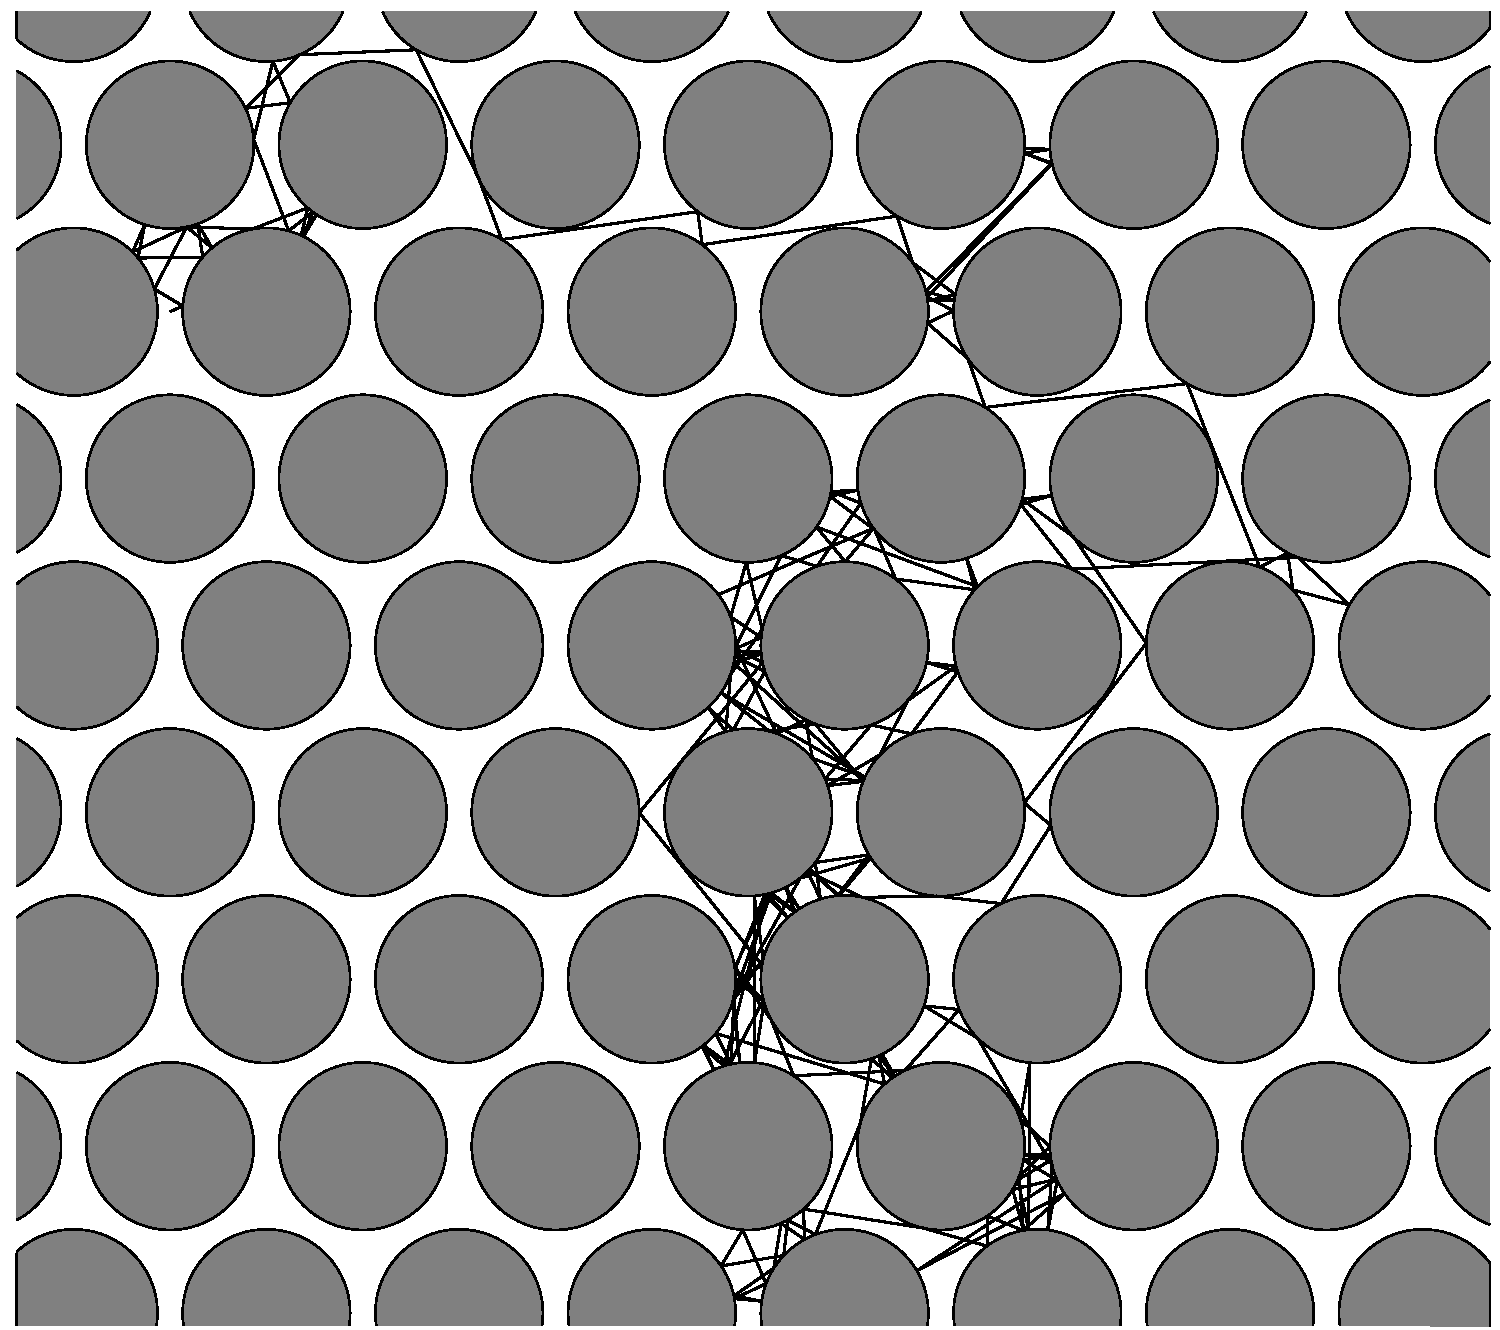
\includegraphics[width=0.45\textwidth]{diffuseChaoticBouncing}
\end{center}
\caption[]{\label{fig-chaoticBouncing}
    Chaos in the Lorentz gas system. A ``gas'' particle is bouncing in
    the array of disks arranged in a hexagonal lattice pattern. The
    distance between the disks are close enough such that the particle
    has no infinite free flight (finite horizon). }
\end{figure}

\begin{figure}[htbp]
\begin{center}
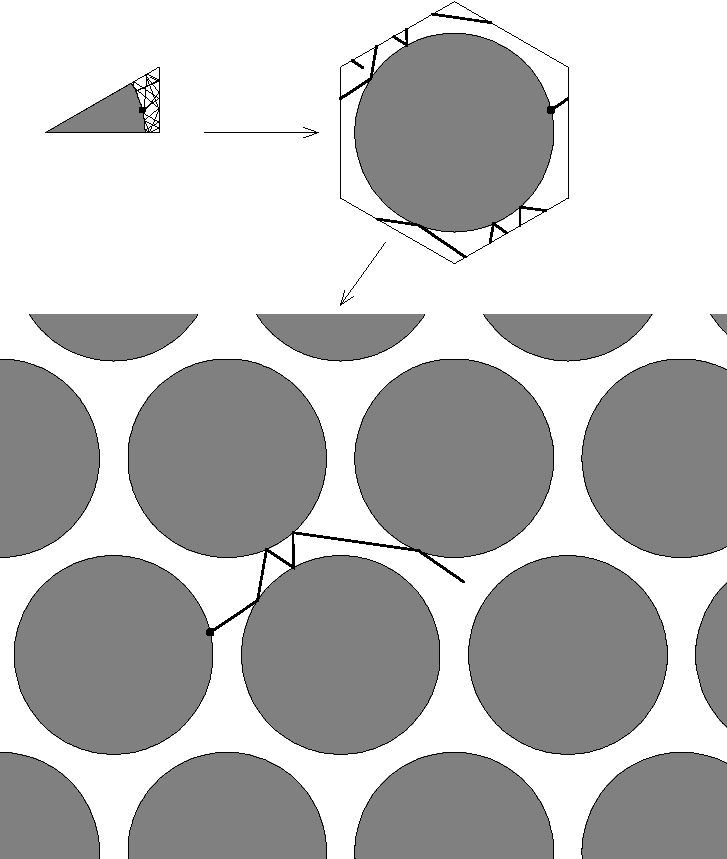
\includegraphics[width=0.45\textwidth]{diffuseSchreiberFig1}
\end{center}
\caption[]{\label{fig-schrieberFig1}
    Motion in fundamental domain (top left), elementary cell (top right)
    and in full space (bottom).}

\end{figure}

The $2$\dmn\ Lorentz gas is an infinite scatterer array in which
diffusion of a light molecule in a gas of heavy scatterers is modeled by
the motion of a point particle in a plane bouncing off an array of
reflecting disks. The Lorentz gas is called ``gas'' as one can
equivalently think of it as consisting of any number of point-like fast
``light molecules'' interacting only with the stationary ``heavy
molecules'' and not among themselves.  As the scatterer array is built up
from only defocusing concave surfaces, it is a pure hyperbolic system,
and one of the simplest nontrivial dynamical systems that exhibits
deterministic diffusion, \reffig{fig-chaoticBouncing}.

% The original Lorentz gas assumed a random distribution of heavy
% scatterers; in this case a probabilistic description is unavoidable.
\subsection{Formulation of Cycle Expansion Theory}
In \refref{CGS92} we have shown that the {\em  periodic} Lorentz  gas is
amenable to a purely deterministic treatment, and have derived the cycle
expansion formula to calculate global dynamical quantities such like
Lyapunov exponent and diffusion coefficient, using dynamics in the
elementary cell. For any dynamical system that has translational
symmetry, the full state space $\hM$ (i.e., both spatial coordinates and
momenta) has a periodic tiling \[\hM=\bigcup_{ \hn \in T} \pS_{\hn},\] by
{\em translating} $\pS_{\hn}$ of an {\em elementary cell} $\pS$, with $T$
the abelian group of lattice translations.

In the context of Lorentz gas system, the elementary cell is the hexagon
region (\reffig{fig-schrieberFig1}) centered at the scatterer. The
dynamics restricted inside the elementary cell is understood as the
periodic boundary condition: when the particle leaves the edge of the
hexagon cell, it immediately enters the region again from the opposite
edge. We distinguish two types of diffusive behavior; the {\em infinite
horizon} case, which allows for infinite length flights, and the {\em
finite horizon} case, where any free particle trajectory must hit a disk
in finite time. The transition between horizon and infinite horizon is
controlled by the ratio of $w/r$, where $w$ is the gap between nearest
pair of disk and $r$ the radius of the disk.

We shall now relate the dynamics in $\pS$ to diffusive properties of the Lorentz gas in $\hM$. Let $\hx(t)\,=\,\hflow{}{\hx_0}$ denotes the point in the global space $\hM$ reached by the flow in time $t$. $x(t)\,=\,\flow{}{\xInit}$ denotes the corresponding flow in the elementary cell; the two are related by
\beq
\hn_t(\xInit)= \hflow{\xInit} - \flow{\xInit} \in T
\,,
\ee{l-diff-hatn}
the translation of the endpoint of the global path into the elementary cell $\pS$.

Fix a vector $\beta \in \reals^d$, where $d$ is the dimension of the {\statesp}. We will compute the diffusive properties of the Lorentz gas from the leading eigenvalue of the Rulle-Frobenius-Perron \evOper\
\beq
\eigenvL(\beta)\,=\, \lim_{t \rightarrow \infty} \frac{1}{t} \log
\langle e^{\beta \cdot (\hx(t) -x) } \rangle_\pS
~, \quad
\ee{lor-diff-1}
where the average is over all initial points in the elementary cell, $x \in \pS$. %, $\tx \in {\widetilde \pS}$ respectively.

If all odd derivatives vanish by symmetry, there is no drift and the second derivatives
\[
2d D_{ij} =
\left . {{\partial} \over {\partial \beta_i}}
{{\partial} \over {\partial \beta_j}}
\eigenvL(\beta)\right |_{\beta=0} \,=\,\lim_{t\rightarrow \infty} {1\over t}
\langle {(\hx(t) -x)_i (\hx(t) -x)_j } \rangle_\pS ~,
\]
yield a diffusion matrix.  This symmetric matrix can, in general, be anisotropic (\ie, have $d$ distinct eigenvalues and eigen\-vectors). The spatial diffusion constant is then given by the Einstein relation
\[
D\,=\,{1\over 2 d} \sum_i
\left .{{\partial}^2 \over {\partial \beta^2_i}}
\eigenvL(\beta)\right |_{\beta=0}
\,=\, \lim_{t\rightarrow \infty} {1\over{2d t}}
\langle {(\hat{q}(t) -q)^2 } \rangle_\pS~
~,
\]
where the $i$ sum is restricted to the spatial components $q_i$ of the {\statesp} vectors $x=(q,p)$, \ie, if the dynamics is Hamiltonian, the sum is over the $d$ degrees of freedom.

% PC{reinstate mass, velocity, size to get $\beta$, $m$, $\sigma dependencies right}

We now turn to the connection between \refeq{lor-diff-1} and periodic orbits in the elementary cell, which is given by the spectrum of the operator
\beq
\det(\eigenvL (\beta) - \Aop)  \,=\,\prod_{p}
\exp \left( - {
               \sum_{r=1}^\infty {1 \over r}
               {
                e^{(\beta \cdot \hn_p- s \period{p}) r}
                    % z^{\cl{p} r}
 \over  \oneMinJ{r}
                }
  % { | \det \left( {\bf 1}-\monodromy_p^{r} \right) | } }
              } \right)
\,,
\ee{lor-diff-14}
or the corresponding \dzeta\
\beq
1/\zeta(\beta, s)\,=\,\prod_{p}\left( 1 - \frac{e^{(\beta \cdot
\hn_p- s \period{p})}}{|\ExpaEig_p|} \right)
~.
\label{zeta-diff}
\eeq
The \dzeta\ \cycForm\ for the diffusion constant, zero mean drift
$
\expct{ \hat{x}_i } = 0
\,,
$
is given by
\beq
D \,=\,{1 \over 2 d} { \expct{\hat{x}^2}_\zeta \over \expct{\period{}}_\zeta }
  \,=\,{1 \over 2 d } \, {1 \over \expct{\period{}}_\zeta}
  \sumprime \frac{(-1)^{k+1}
  (\hn_{p_1}+ \cdots+ \hn_{p_k})^2}
  {|\ExpaEig_{p_1}\cdots \ExpaEig_{p_k}|}
\, .
\label{(17)}
\eeq
where the sum is over all distinct non-repeating combination of prime cycles (in the elementary cell). The derivation is standard, still the formula is strange. Diffusion is unbounded motion across an infinite lattice; nevertheless, the reduction to the elementary cell enables us to compute relevant quantities in the usual way, in terms of periodic orbits.

\subsection{Cycles in Elementary Cell}
\begin{figure}
\begin{center}
(a)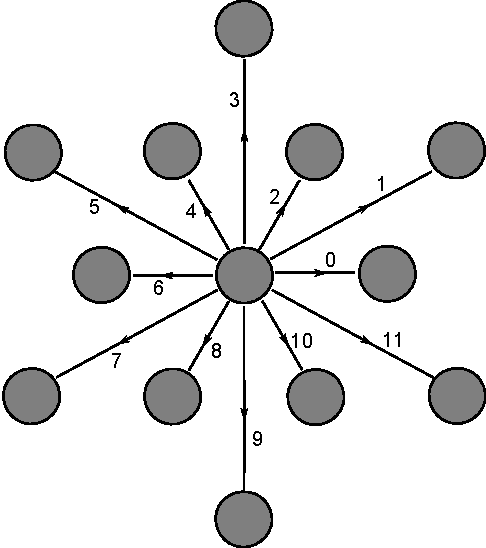
\includegraphics[width=0.45\textwidth]{diffuseDiskDirectionsElCell}
(b)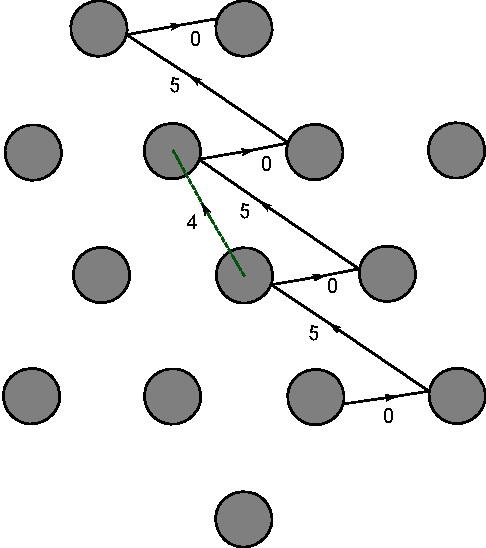
\includegraphics[width=0.45\textwidth]{diffuseDiskDirecsElCell05}
(c)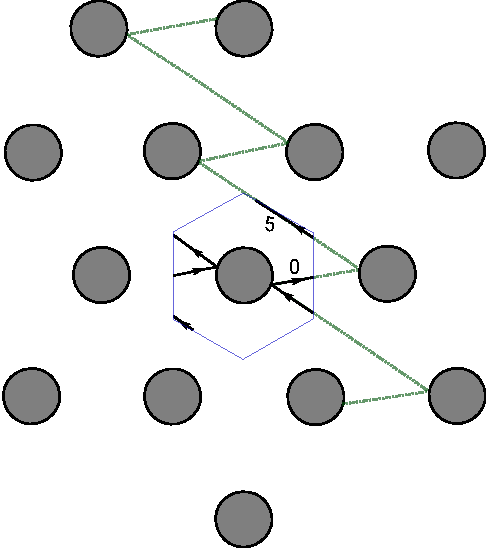
\includegraphics[width=0.45\textwidth]{diffuseDiskDirecsElCell05red}
\end{center}
\caption{
Elementary cell symbolic dynamics is obtained by labeling the translation vectors connecting the center of the current disk to the center of the next disk. (a) The finite horizon is here imposed by limiting jumps from the center cell to only the short jumps (six even labels $0, 2,\cdots,10$) and the `long jumps' (six odd labels $1, 3,\cdots,11$). (b) Running mode \cycle{05} advances by $\hn_4$ per period. (c) In the elementary cell this is a \po\ \cycle{05}
    of topological length 2.
    }
\label{fig-diskDirectionsElCell}
\end{figure}

We will use the same symbolic dynamics developed in \refref{CGS92} and only briefly outline the concepts here. With imposed finite horizon there are 12 possible ways of jump from one disk to another(~\reffig{fig-diskDirectionsElCell}).


\section{Into the fundamental domain\label{s-SymmetryReduction}
}

 When the scattering array has further discrete symmetries, such as reflection symmetry, each elementary cell may be built from a {\em fundamental domain} ${\widetilde \pS}$ by the action of a discrete (not necessarily abelian) group $G$. The quantity $\tx(t)\,=\,\tflow{t}{\tx}$ denotes the flow in the fundamental domain ${\widetilde \pS}$; $\tflow{t}{\tx}$ is related to $\flow{}{\tx}$ by a discrete symmetry $g \in G$ which maps $\tx(t)\in {\widetilde \pS}$ to ${x}(t) \in {\pS}$. The full $\hM \rightarrow {\widetilde \pS}$ reduction is complicated by the non-abelian nature of $G$, and will be illustrated in this section in detail.


\begin{figure}[htbp]
\begin{center}
(a)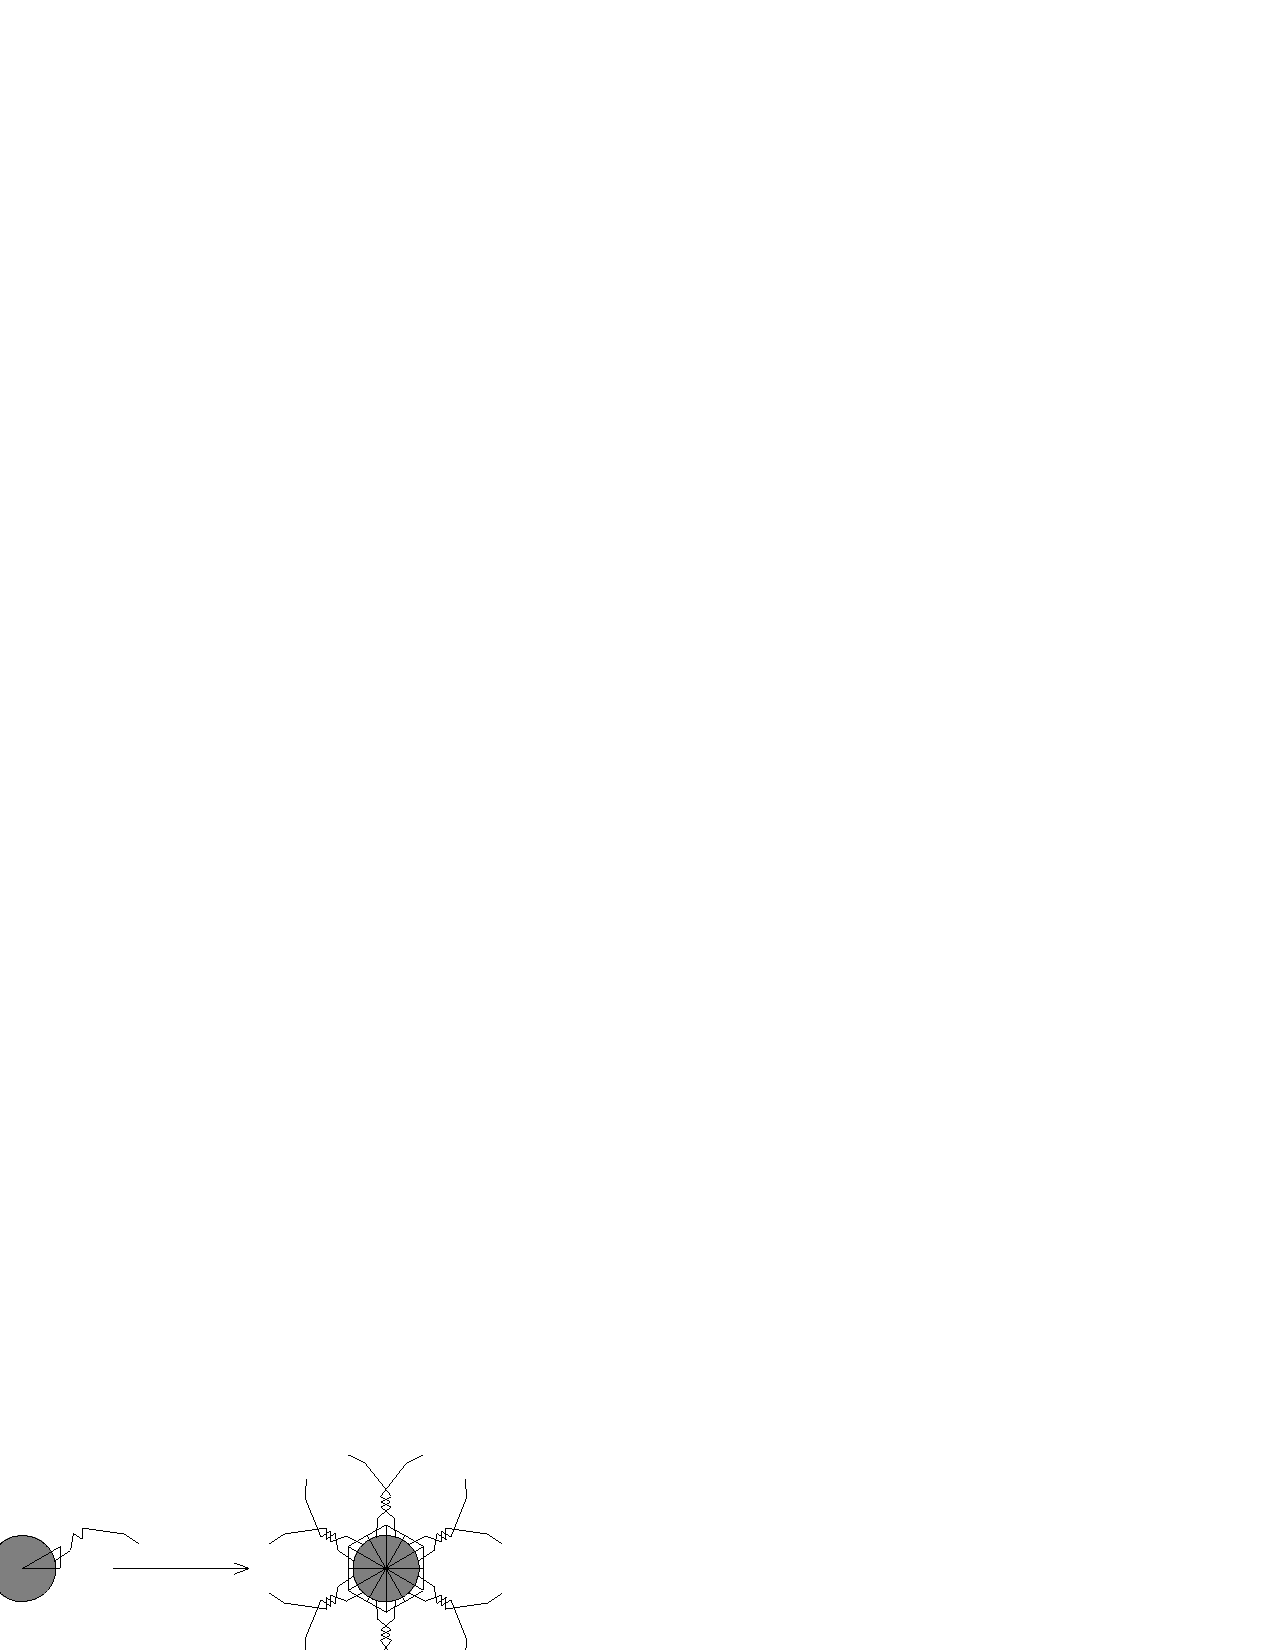
\includegraphics[width=0.45\textwidth]{diffuseSchreiberFig2}
(b)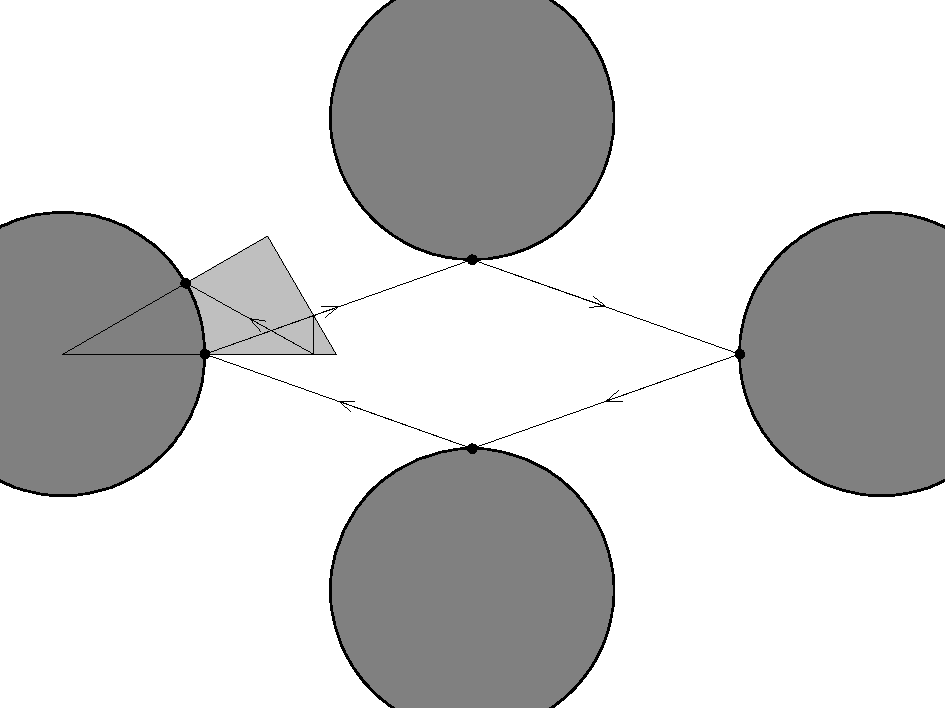
\includegraphics[width=0.45\textwidth]{diffuseSchreiberFig3}
\end{center}
\caption[]{ \label{fig:schrieberFig23}
(a) An (unwrapped) trajectory (in full space) and its 12 copies after applying point group actions to it. (b) Multiplicity of periodic orbits in fundamental domain.}
\end{figure}

\subsection{How point group changes translation}


In fundamental domain, one has to realize a few things to proceed the cycle expansion derivation. 

The first thing is about G-equivariance of displacement under point group actions, which connects the displacement in full space when starting from elementary cell and fundamental domain. 

Also, one notice that after traveling along a fundamental domain cycle once, the displacement in full space depends on where we start from on the cycle.  

\subsection{Gymnastics of equations}

\Group-equivariance of the displacement in the full space.

\begin{align}
\tr{\cal L}^t &= \sum_{\alpha \in\II_G} \tr{\cal L}_{\alpha}^t\nonumber\\
\tr{\cal L}_{\alpha}^t &= \frac{d_\alpha}{|G|}\sum_{\sigma \in G}\sum_{h\in G}\chi_\alpha(h)\int_{\t {\cal M}} d\tx \delta (h\tx - f^t(\tx))e^{\beta\cdot\sigma\cdot\hphi^t(\tx)}~,
\label{e1}
\end{align}

\begin{align}
\frac{1}{\zeta_{\alpha}(\beta,s,z)} &=\exp\left(-\frac{d_\alpha}{|G|}\sum_{\sigma\in G}\sum_{\tp}\frac{1}{n_{\tp}}\sum_{\tx_{i}\in\tilde{p}}\sum_{r=1}^{\infty}\frac{t_{\tp}^{r}}{r}\chi_{\alpha}(\hp^{r}(\tx_i))e^{\beta\cdot\sigma\cdot\hat{L}_{\tp}(r,\tx_i)}\right)
\end{align}
where we have defined
\begin{equation}
t_{\tp}\equiv \frac{z^{n_{\tp}}e^{-sT_{\tp}}}{|\ExpaEig_\tp|}
\end{equation}
and
\begin{equation}
\hat{L}_{\tp}(r,\tx_i)\equiv (e+\hp^{-1}(\tx_i)\cdots+\hp^{-r+1}(\tx_i))\cdot\hn_{\tp}(\tx_i)
\end{equation}

We are interested in the one dimensional, symmetric trivial representation with $ d_\alpha = 1 $ and all $ \chi(h) = 1 $,; there by we drop the subscript $ \alpha $ in the following calculation. Partial derivative with respect to $\beta$:
\bea
\frac{\partial^{2}}{\partial\beta^{2}}\frac{1}{\zeta(\beta,s,z)}
 &=\frac{1}{\zeta(\beta,s,z)}\left(\left(\frac{1}{|G|} \sum_{\sigma\in G}\sum_{\tp}\sum_{\tx_i\in \tp}\sum_{r=1}^{\infty}\frac{\sigma\cdot \hat{L}_{\tp}(r,\tx_i)t_{\tp}^r e^{\beta\cdot\sigma\cdot \hat{L}_{\tp}(r,\tx_i)}}{n_{\tp}r}\right)^{2}\right.\nonumber\\
 & \left.-\frac{1}{|G|}\sum_{\sigma\in G}\left(\sum_{\tp}\sum_{\tx_i\in \tp}\sum_{r=1}^{\infty}\frac{\vert \sigma\cdot \hat{L}_{\tp}(r,\tx_i)\vert^{2}t_{\tp}^{r}e^{\beta\cdot\sigma\cdot \hat{L}_{\tp}(r,\tx_i)}}{n_{p}r}\right)\right).
\eea
The first term in the formula corresponds to $ \langle\hx\rangle^2 $ and second to $ \langle\hx^2\rangle $

\subsection{Grammar of Fundamental Domain cycle}
\begin{figure}[tbp]
(a)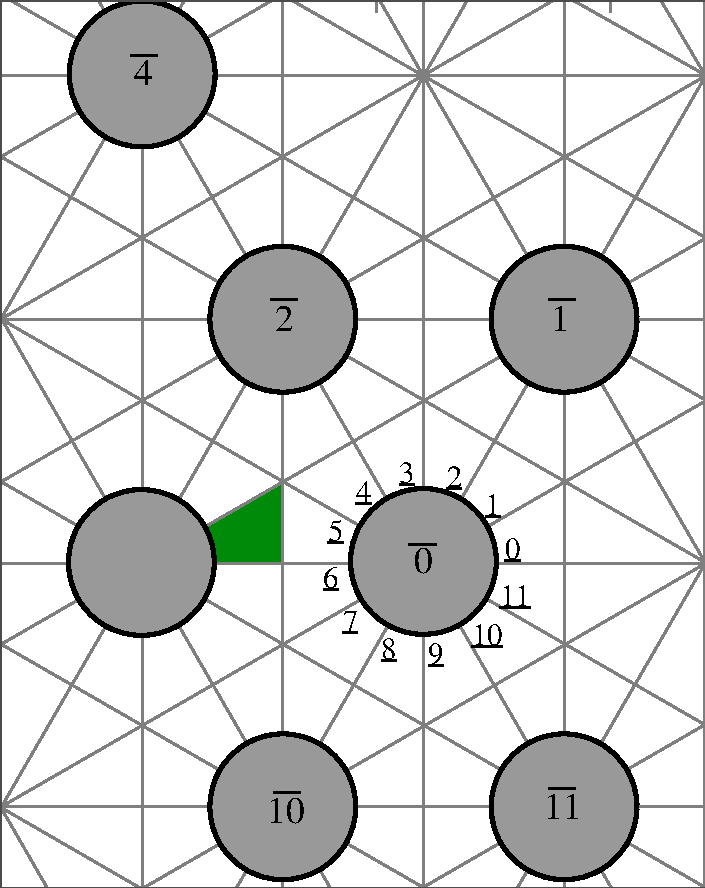
\includegraphics[width=0.45\textwidth]{diffuseFDSymbolIllustration}
(b)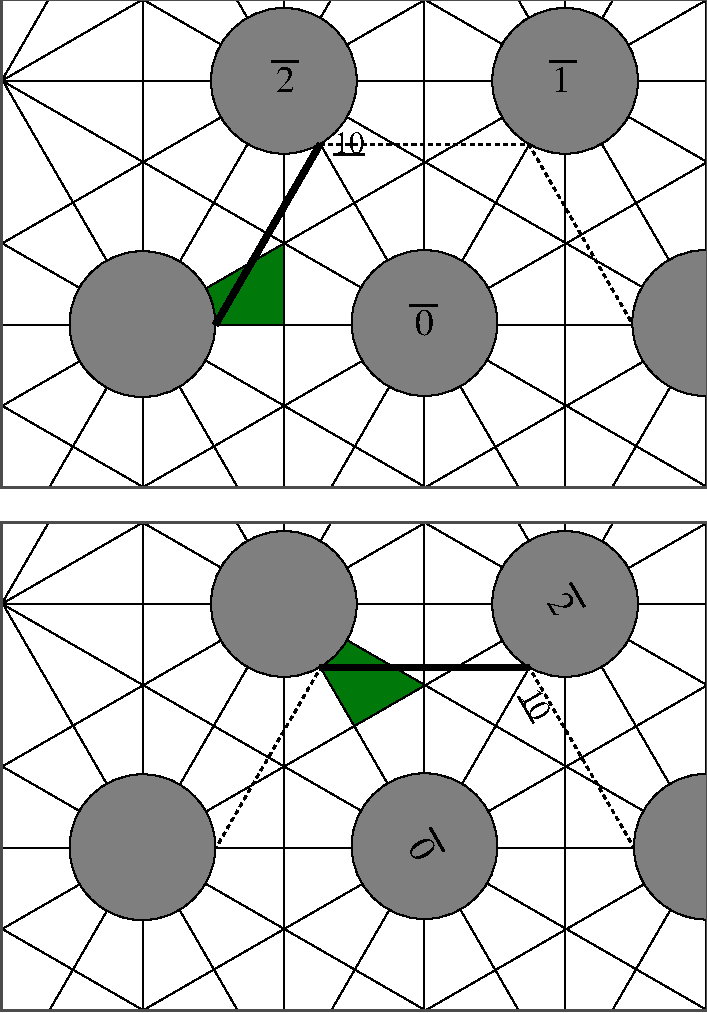
\includegraphics[width=0.45\textwidth]{diffuseFDSymbolOrbits}

\caption{\label{fig-fdflights} Fundamental domain symbolic dynamics. (a) With imposed finite horizon and starting on the edge of a disk in fundamental domain (the green filled region), there are at most 6 disks can be reached without collision (disk $\overline{0},\overline{1},\overline{2},\overline{4},\overline{10}$ and $\overline{11}$). Similar to how elementary cell symbolic dynamics are created, we label the 12 triangular pieces of a disk in a counter clock-wise manner, from $\underline{0}$ to $\underline{11}$. The combination of a disk label and a triangular piece label $\{\overline{i},\underline{j}\}$ uniquely identifies a free flight. (b) The fundamental domain fixed point $\{\overline{2},\underline{10}\}$, which corresponds to a periodic orbit of length 6 in elementary cell ($\cycle{0246810}$), is unwrapped in global space. After each collision we re-label the disks and triangular partitions according their relative positions to the ``new'' fundamental domain. In the figure the labels are also rotated according to the point group actions.}
\end{figure}

\begin{figure}
\begin{center}
(a) \includegraphics[width=0.45\textwidth]{7diskFundDflips}
(b) \includegraphics[width=0.45\textwidth]{7diskFundDtiles}
\end{center}
\caption{\label{fig-7diskFundDflips} (a) The three generators of tiling of the plane by a fundamental domain: two generators of \Dn{12} tiling, reflection $s$ across the short disk-disk separation, reflection  $\ell$  across the long disk-disk separation; and a translation generator $f$ that pivots (`flips') a disk center to disk center by flip across the symmetry line normal to the short disk-disk separation. (5) Tiling of the 7-disk by copies of the fundamental domain, labelled by a (not unique) sequence of the three generators $\{s,\ell,f\}$, chosen so that each sequence contain one and only on disk-to-disk pivot $f$. }
\end{figure}
XX I do not really use the three generators to compute the FD domain cycles, instead I use the idea of topological flights (\reffig{fig-fdflights}).


\section{Results and Discussions}

\begin{table}[htbp]
{\small
%\begin{center}
\begin{tabular}{|r|r|r|l|l|}
\hline
$\period{p}$ & \# cycles & $\zeta$(0,0) & $\lambda$ & D \\ \hline\hline
1      & 0      &   -    &   -  &   - \\
2      & 24     & -0.31697 & 1.330 & 0.375\\
3      & 64     & -0.54152 & 1.435 & 0.339\\
4      & 168    & -0.09764 & 1.902 & 0.284\\
5      & 516    &  0.02334 & 2.324 & 0.215\\
6      & 1589   & -0.00481 & 1.975 & 0.133\\
7      & 5700   & -0.01241 & 1.885 & 0.184\\
8      & 20729  & -0.01006 & 1.785 & 0.247\\ \hline\hline
\multicolumn{4}{|l|}{numerical experiment} 1.760 & 0.25 \\ \hline
\end{tabular}
\hfill
\begin{tabular}{|r|r|r|l|l|}
\hline
$\period{p}$ & \# cycles & $\zeta$(0,0) & $\lambda$ & D \\ \hline\hline
1      & 5      &   -0.2169759    &   1.39193  &   0.37795 \\
2      & 10     & -0.0248233 & 1.74541 & 0.23118\\
3      & 33     & -0.0221962 & 1.72235 & 0.25257\\
4      & 108    & -0.0002192 & 1.74450 & 0.24165\\
5      & 373    &  0.0023463 & 1.76079 & 0.24468\\
6      & 1378   &  0.0096330 & 1.75610 & 0.24068\\ \hline\hline
\multicolumn{3}{|l|}{numerical experiment}
                           & 1.760 & 0.25
\\ \hline
\end{tabular}
}

\caption{\label{TCELL2}
Results for $w$=0.3. (left) Schreiber 1992 calculation\rf{CGS92} (and
this paper) in EC. (right) Our calculation in FD. Gaspard 1992
note: ``My numerical estimate for the Lyapunov exponent when $w=0.3$ is
$\lambda = 1.760 \pm 0.002$, which supports the result of this table.''
}
\end{table}

\begin{figure}
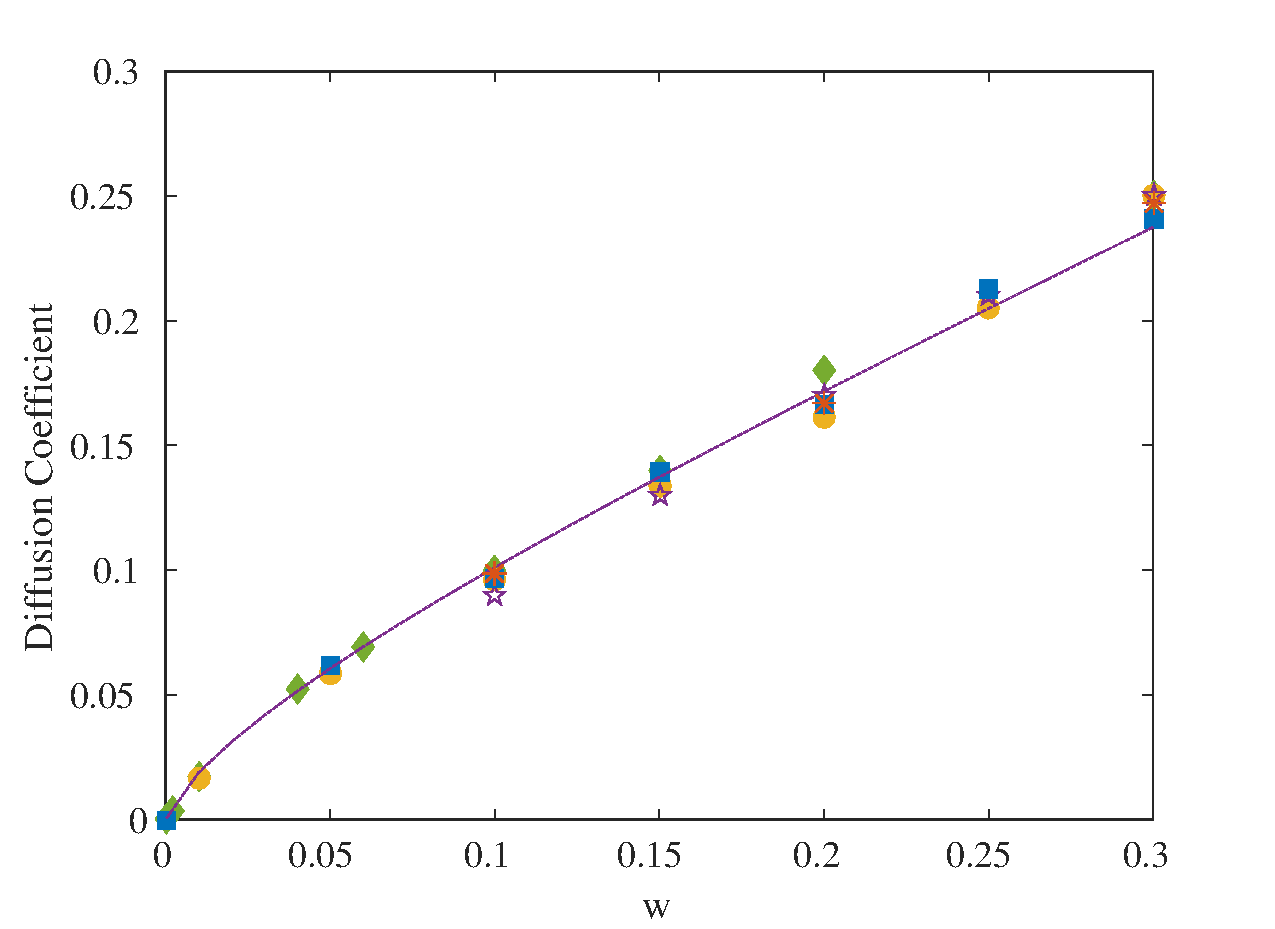
\includegraphics[width=0.45\textwidth]{diffuseDiffCoefPlot}
\caption[]{\label{fig-results} Diffusion coefficients as a function of inter-disk separation distance $w$.}
\end{figure}
% Put \label in argument of \section for cross-referencing
%\section{\label{}}

% If in two-column mode, this environment will change to single-column
% format so that long equations can be displayed. Use
% sparingly.
%\begin{widetext}
% put long equation here
%\end{widetext}

% figures should be put into the text as floats.
% Use the graphics or graphicx packages (distributed with LaTeX2e)
% and the \includegraphics macro defined in those packages.
% See the LaTeX Graphics Companion by Michel Goosens, Sebastian Rahtz,
% and Frank Mittelbach for instance.
%
% Here is an example of the general form of a figure:
% Fill in the caption in the braces of the \caption{} command. Put the label
% that you will use with \ref{} command in the braces of the \label{} command.
% Use the figure* environment if the figure should span across the
% entire page. There is no need to do explicit centering.

% \begin{figure}
% \includegraphics{}%
% \caption{\label{}}
% \end{figure}

% Surround figure environment with turnpage environment for landscape
% figure
% \begin{turnpage}
% \begin{figure}
% \includegraphics{}%
% \caption{\label{}}
% \end{figure}
% \end{turnpage}

% tables should appear as floats within the text
%
% Here is an example of the general form of a table:
% Fill in the caption in the braces of the \caption{} command. Put the label
% that you will use with \ref{} command in the braces of the \label{} command.
% Insert the column specifiers (l, r, c, d, etc.) in the empty braces of the
% \begin{tabular}{} command.
% The ruledtabular enviroment adds doubled rules to table and sets a
% reasonable default table settings.
% Use the table* environment to get a full-width table in two-column
% Add \usepackage{longtable} and the longtable (or longtable*}
% environment for nicely formatted long tables. Or use the the [H]
% placement option to break a long table (with less control than
% in longtable).
% \begin{table}%[H] add [H] placement to break table across pages
% \caption{\label{}}
% \begin{ruledtabular}
% \begin{tabular}{}
% Lines of table here ending with \\
% \end{tabular}
% \end{ruledtabular}
% \end{table}

% Surround table environment with turnpage environment for landscape
% table
% \begin{turnpage}
% \begin{table}
% \caption{\label{}}
% \begin{ruledtabular}
% \begin{tabular}{}
% \end{tabular}
% \end{ruledtabular}
% \end{table}
% \end{turnpage}

% Specify following sections are appendices. Use \appendix* if there
% only one appendix.
%\appendix
%\section{}

% If you have acknowledgments, this puts in the proper section head.
%\begin{acknowledgments}
% put your acknowledgments here.
%\end{acknowledgments}

\bibliography{../bibtex/siminos,../bibtex/diffuse}

        \ifboyscout
%\PublicPrivate{}{% switch \PublicPrivate{
\newpage
\input ../tingnan/flotsam
%      }% end \PublicPrivate{


\end{document}
%
% ****** End of file apstemplate.tex ******
